\documentclass[../report.tex]{subfiles}
\graphicspath{{\subfix{../image/}}}

\begin{document}
\maketitle

\section*{HX711 Interface Module and Load cell}

Definition: A Load Cell serves as a sensor that transforms applied force, encompassing pressure, rotational force, compression, or tension, into quantifiable electrical signals.
The load cell generates an output in millivolt range; therefore, it is essential to magnify this signal into a higher-level amplitude and subsequently convert it into a digital format for further processing.
To accomplish this task, we employ the HX711 interface module. This module serves to amplify the load cell's low-voltage output and transmit it to the Arduino for weight calculation. 
The illustration below depicts the HX711 interface module.


\begin{figure}[h!]
    \centering
    \begin{subfigure}[b]{0.4\linewidth}
      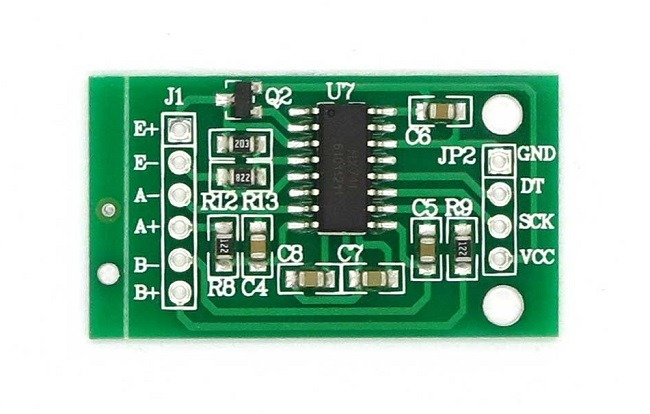
\includegraphics[width=\linewidth]{image/HX711-Weighing-Sensor-Dual-Channel-24-Bit-Precision-A-D-Module-Pressure-Sensor_1.jpg}
      \caption{HX711 Interface Module }
    \end{subfigure}
    \begin{subfigure}[b]{0.4\linewidth}
      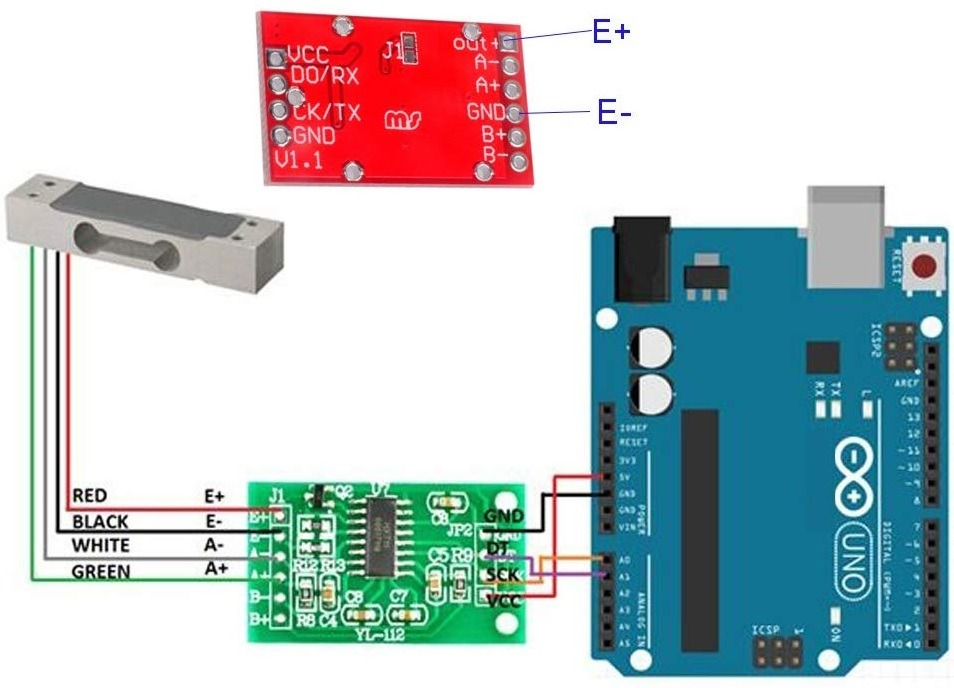
\includegraphics[width=\linewidth]{image/hx711-red.jpg}
      \caption{HX711 Interface Module and Load cell using Arduino}
    \end{subfigure}
    
    
  \end{figure}
  
\end{document}